\begin{figure}[t]
    \centering
    \begin{subfigure}[b]{0.37\linewidth}
        \centering
        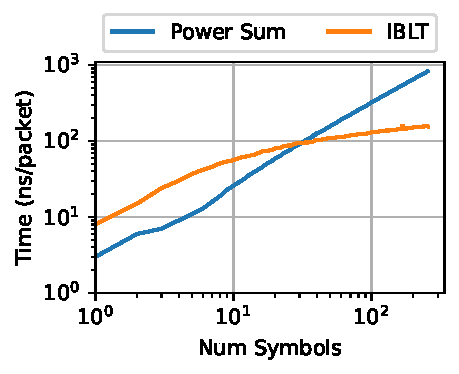
\includegraphics[width=\linewidth]{quack/figures/quack_encode.pdf}
        \caption{Encode time.}
        \label{fig:quack:iblt-computation:encode}
    \end{subfigure}
    \begin{subfigure}[b]{0.37\linewidth}
        \centering
        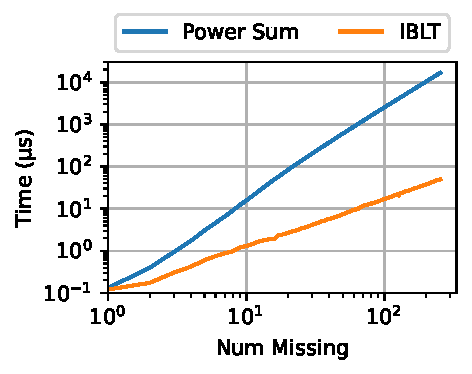
\includegraphics[width=\linewidth]{quack/figures/quack_decode.pdf}
        \caption{Decode time.}
        \label{fig:quack:iblt-computation:decode}
    \end{subfigure}
    \caption{IBLT vs. power sum quACK microbenchmarks. The IBLT quACK is more
     computationally scalable than the power sum quACK, but the encoding time
     suffers from constant factor overheads with a smaller number of symbols.
     The cumulative time of the trials is at least $100$ ms.
     }
    \label{fig:quack:iblt-computation}
\end{figure}